% Created 2023-05-28 Sun 21:55
% Intended LaTeX compiler: pdflatex
\documentclass[11pt]{article}
\usepackage[utf8]{inputenc}
\usepackage[T1]{fontenc}
\usepackage{graphicx}
\usepackage{longtable}
\usepackage{wrapfig}
\usepackage{rotating}
\usepackage[normalem]{ulem}
\usepackage{amsmath}
\usepackage{amssymb}
\usepackage{capt-of}
\usepackage{hyperref}
\author{Krzysztof Szczerbowski}
\date{\today}
\title{Raport - Optymalizacja Baz Danych\\\medskip
\large Wirtualny rynek graczy i postaci niezależnych}
\hypersetup{
 pdfauthor={Krzysztof Szczerbowski},
 pdftitle={Raport - Optymalizacja Baz Danych},
 pdfkeywords={},
 pdfsubject={},
 pdfcreator={Emacs 28.2 (Org mode 9.5.5)}, 
 pdflang={English}}
\begin{document}

\maketitle
\tableofcontents


\section{Struktura bazy danych}
\label{sec:org84076f9}
Przyjęta struktura bazy danych została zaprezentowana na poniższej ilustracji:
\begin{center}
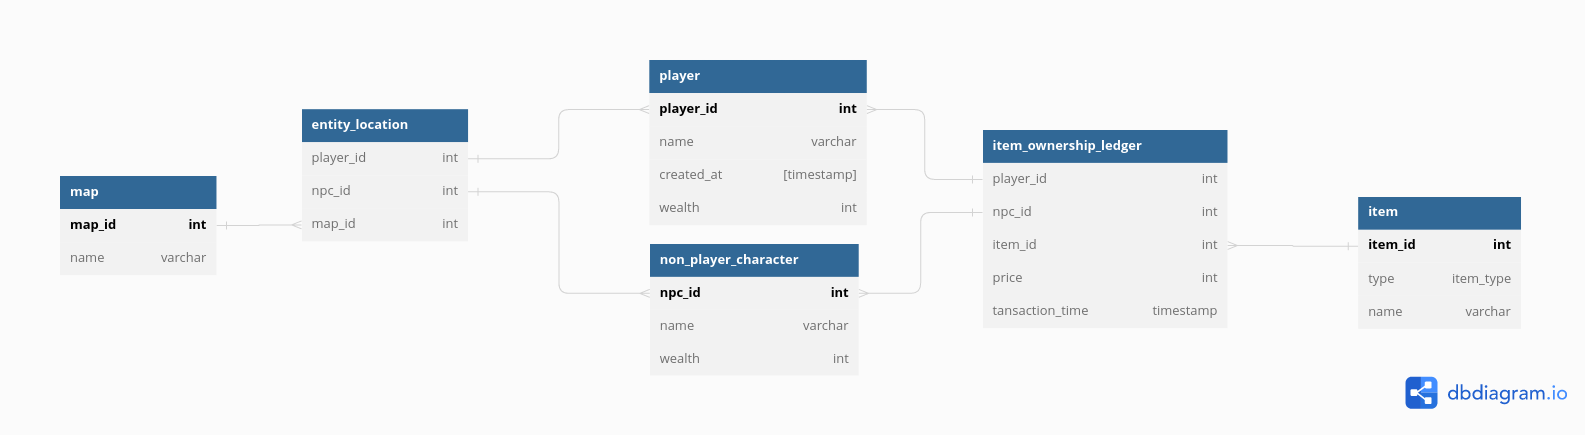
\includegraphics[width=.9\linewidth]{./structure/mmo-backbone.png}
\end{center}

\section{Generowanie danych}
\label{sec:orgb48d85c}
Elementy tablic \texttt{map}, \texttt{player}, \texttt{non\_player\_character}, oraz \texttt{item} zostały wygenerowane na
podstawie liczb pseudo losowych. Elementy tablic \texttt{entity\_location} i \texttt{item\_ownership\_ledger}
zostały wygenerowane na podstawie danych z wyżej wymienionych tablic.

\subsection{\texttt{map}}
\label{sec:org7ff6e76}
\begin{verbatim}
create or replace procedure create_maps as
  rseed number(20);
  map_name varchar2(32);
  last_pk number(38,0);
  cnt number;
begin
  -- initizalize dbms random with rseed
  select to_number(to_char(sysdate, 'sssss')) into rseed from dual;
  dbms_random.initialize(rseed);

  -- determine last pk if ther is any
  select count(*) into cnt from map;
  if(cnt = 0)
  then
    select 0 into last_pk from dual;
  else
    select max(map_id) into last_pk from map;
  end if;

  -- random map (map_id, name)
  for i in 1..100
  loop
    -- name
    map_name := dbms_random.string('L', trunc(dbms_random.value(4,32)));

    -- generated map
    insert into map values(last_pk+i, map_name);
  end loop;

end create_maps;
\end{verbatim}

\subsection{\texttt{player}}
\label{sec:orgdba02c9}
\begin{verbatim}
create or replace NONEDITIONABLE procedure create_users as
  rseed number(20);
  user_name varchar2(32);
  created_at timestamp;
  wealth number(38);
  last_pk number(38,0);
  cnt number;
begin
  --dbms_output.enable();
  --dbms_output.put_line('Create users procedure');

  -- initizalize dbms random with rseed
  select to_number(to_char(sysdate, 'sssss')) into rseed from dual;
  dbms_random.initialize(rseed);

  -- determine last pk if ther is any
  select count(*) into cnt from player;
  if(cnt = 0)
  then
    select 0 into last_pk from dual;
  else
    select max(player_id) into last_pk from player;
  end if;
  --dbms_output.put_line('Last player_id: '||last_pk);

  -- random player (player_id, name, created_at, wealth)
  for i in 1..10
  loop
    -- player_id; simply the 'i' from for

    -- name
    user_name := dbms_random.string('L', trunc(dbms_random.value(6,32)));
    --dbms_output.put_line(user_name);

    -- created_at timestamp
    select to_date(sysdate - 1000,'YY-MM-DD HH24:MI:SS')+dbms_random.value(0, 100) into created_at from dual;
    --dbms_output.put_line(created_at);

    -- wealth
    wealth := dbms_random.value(1,38);
    --dbms_output.put_line(wealth);

    -- generated player data
    --dbms_output.put_line('player: ' || (last_pk+i) ||' '|| user_name ||' '|| created_at ||' '|| wealth);

    -- insert into the player table
    insert into player values(last_pk+i, user_name, created_at, wealth);
  end loop;

end create_users;
\end{verbatim}

\subsection{\texttt{non\_player\_character}}
\label{sec:orga7ba462}
\begin{verbatim}
create or replace procedure create_npcs as
  rseed number(20);
  npc_name varchar2(32);
  wealth number(38,0);
  last_pk number(38,0);
  cnt number;
begin
  --dbms_output.enable();
  --dbms_output.put_line('Create users procedure');

  -- initizalize dbms random with rseed
  select to_number(to_char(sysdate, 'sssss')) into rseed from dual;
  dbms_random.initialize(rseed);

  -- determine last pk if ther is any
  select count(*) into cnt from non_player_character;
  if(cnt=0)
  then
    select 0 into last_pk from dual;
  else
    select max(npc_id) into last_pk from non_player_character;
  end if;
  --dbms_output.put_line('Last npc_id: '||last_pk);

  -- random npc (npc_id, name, wealth)
  for i in 1..1000
  loop
    -- npc_id; simply the 'last_pk+i' from for

    -- name
    npc_name := dbms_random.string('L', trunc(dbms_random.value(6,32)));
    --dbms_output.put_line(user_name);

    -- wealth
    wealth := dbms_random.value(1,38);
    --dbms_output.put_line(wealth);

    -- generated player data
    --dbms_output.put_line('npc: ' || (last_pk+i) ||' '|| npc_name ||' '|| wealth);

    -- insert into the player table
    insert into non_player_character values(last_pk+i, npc_name, wealth);
  end loop;

end create_npcs;
\end{verbatim}

\subsection{\texttt{item}}
\label{sec:org1818239}
\begin{verbatim}
create or replace procedure create_items as
  rseed number(20);
  item_name varchar2(32);
  item_type number(2); -- 0: non-tradable; 1: consumable; 2: bind type
  last_pk number(38,0);
  cnt number;
begin
  -- initizalize dbms random with rseed
  select to_number(to_char(sysdate, 'sssss')) into rseed from dual;
  dbms_random.initialize(rseed);

  -- determine last pk if ther is any
  select count(*) into cnt from item;
  if(cnt = 0)
  then
    select 0 into last_pk from dual;
  else
    select max(item_id) into last_pk from item;
  end if;

  --dbms_output.enable();

  -- random item (item_id, item_type, name)
  for i in 1..100000
  loop
    -- type
    item_type := dbms_random.value(0,2);

    -- name
    item_name := dbms_random.string('L', trunc(dbms_random.value(3,32)));

    -- generated item
    --dbms_output.put_line('item: '||(last_pk+i)||' '||item_type||' '||item_name);
    insert into item values(last_pk+i, item_type, item_name);
  end loop;

end create_items;
\end{verbatim}

\subsection{\texttt{entity\_location}}
\label{sec:org8ea4f2a}
Elementy tablicy \texttt{entity\_location} zawierają informację o zależności (położeniu)
danych z tablic \texttt{player} oraz \texttt{non\_player\_character} i dane te posiadają rozkład normalny.
\begin{verbatim}
create or replace NONEDITIONABLE procedure populate_location as
  rseed number(20);
  rand_map number(38,0);
  r1 number(38, 0);
  r2 number(38, 0);
  max_map_id number(38,0);
  player_id number(38,0);
  npc_id number(38,0);
begin
  --dbms_output.enable();

  -- initialize dbms random with rseed
  select to_number(to_char(sysdate, 'sssss')) into rseed from dual;
  dbms_random.initialize(rseed);

  -- max map id pk
  select max(map_id) into max_map_id from map;

  -- put players into random locations (pseudo normal distribution)
  begin
  for player_rec in (select player_id from player)
  loop
    -- random map id
    r1 := dbms_random.value(1, (max_map_id/2));
    r2 := dbms_random.value(1, (max_map_id/2));
    rand_map := to_number(trunc(r1+r2,(max_map_id/2)));

    -- next player id, insert into the table
    player_id := player_rec.player_id;
    insert into entity_location values(player_id, NULL, rand_map);
  end loop;
  end;

  -- put npcs into random locations (pseudo normal distribution)
  begin
  for npc_rec in (select npc_id from non_player_character)
  loop
    -- random map id
    r1 := dbms_random.value(1, (max_map_id/2));
    r2 := dbms_random.value(1, (max_map_id/2));
    rand_map := to_number(trunc(r1+r2,(max_map_id/2)));

    -- next npc into id, insert into the table
    npc_id := npc_rec.npc_id;
    insert into entity_location values(NULL, npc_id, rand_map);
  end loop;
  end;

  dbms_random.terminate;

end populate_location;
\end{verbatim}

\subsection{\texttt{item\_ownership\_ledger}}
\label{sec:org340c0bf}
Elementy tablic \texttt{item\_ownership\_ledger} zostały wygenerowane w następujący sposób:
\begin{verbatim}
-- Próby wykonania transakcji w pętli:
create or replace NONEDITIONABLE procedure convey_transactions as
    in_seed number;
begin
  dbms_output.enable();

  for i in 1 .. 1000
  loop
    BEGIN
	in_seed := i;
	ADD_TRANSACTION(in_seed => in_seed);
	commit;
    END;
  end loop;

end convey_transactions;

create or replace NONEDITIONABLE procedure add_transaction as
    rseed number(20);
    r_player_id number(38, 0);
    r_player_wealth number(38, 0);
    r_player_created_at timestamp;
    r_npc_id number(38, 0);
    r_map_id number(38, 0);
    r_item_id number(38, 0);
    r_price number(38, 0);
    transaction_timestamp timestamp(6);
begin
  -- transaction is a process of buying somethin by a player from an npc
  -- a tranasction can occure if all of the conditions are met:
  -- both entities are in the same map (player and npc),
  -- item of question is tradable (item_type = 1 or item_type = 2),
  -- price of the item is less than or equal to the wealth of the buying entitie (if not, haggle once),
  -- random player has to have creation timestamp from before the transaction timestap
  dbms_output.enable();

  select to_number(to_char(sysdate, 'sssss')) into rseed from dual;
  dbms_random.initialize(rseed);

  -- random value for the price
    r_price := dbms_random.value(1,38);

  -- select random tradable item
    insert into tmp_item select item_id,name from item
    where item_type != 0
    order by dbms_random.random;
    select item_id into r_item_id from tmp_item
    where rownum = 1;

  -- select random player and npc, both have to be in the same location
    insert into tmp_map select * from entity_location order by dbms_random.random;
  -- select random map
    select map_id into r_map_id from tmp_map where rownum = 1;
  -- select random palyer
    select player_id into r_player_id from tmp_map
    where rownum = 1 and map_id = r_map_id and player_id is not null;
  -- select random npc
    select npc_id into r_npc_id from tmp_map
    where rownum = 1 and map_id = r_map_id and npc_id is not null;

  -- prepare transaction timestamp
    select to_date(sysdate-1000, 'YY-MM-DD HH24:MI:SS')+dbms_random.value(-100, 100)
    into transaction_timestamp from dual;

  -- check whether this random player is able to buy the item
  -- wealth vs. price and created at timestamp vs. transaction timestamp
    select wealth,created_at into r_player_wealth,r_player_created_at from player
    where player_id=r_player_id;

  -- if so, then yes, buy the item
  -- substract and add price value accordingly for the player and for the npc
    if r_player_wealth >= r_price and r_player_created_at < transaction_timestamp
    then
	dbms_output.put_line('buy the item');

	-- substract and add price value for the player and for the npc
	update (select wealth from player where player_id = r_player_id)
	set wealth = wealth - r_price;
	update (select wealth from non_player_character where npc_id = r_npc_id)
	set wealth = wealth + r_price;

	-- write the transaction to the ledger
	insert into item_ownership_ledger values(
	    r_player_id, r_npc_id,
	    r_item_id, r_price,
	    transaction_timestamp
	);
    end if;

    --dbms_output.put_line(r_map_id||' '||r_player_id||' '||r_npc_id);

  dbms_random.terminate;
end add_transaction;
\end{verbatim}

\section{Zapytania}
\label{sec:org1d59316}
Na podstawie tak wygenerowanych danych zostały przygotowane trzy zapytania.

\subsection{Przedmioty gracza}
\label{sec:orgf2829a3}
Pierwsze zapytanie zostało ograniczone do złożonej instrukcji \texttt{select}.
Zapytanie odpowiada na pytanie \emph{jakie przedmioty posiada (pseudo) losowo wybrany gracz
na podstawie informacji zawartych w} \hyperref[sec:org340c0bf]{\texttt{item\_ownership\_ledger}} \emph{?}
\begin{verbatim}
-- select all (random) player's items which were obtaind in transactions
-- with the:
-- * seller of the item (an npc)
-- * item id
-- * type of the item
-- * value of the transaction
-- * timestamp of acquisition of each of the items
select item_ownership_ledger.player_id,
      item_ownership_ledger.npc_id,
      item_ownership_ledger.item_id, item.item_type,
      item_ownership_ledger.price,
      item_ownership_ledger.transaction_time
from item_ownership_ledger
left join item on item_ownership_ledger.item_id = item.item_id
where player_id =
    (select player_id from (
	select player_id
	from item_ownership_ledger
	order by dbms_random.random
	) where rownum = 1
    )
\end{verbatim}

\subsection{Transakcje wybranej postaci niezależnej}
\label{sec:org134c64a}
Drugie zapytanie zostało przygotowane w postaci procedury korzystającej z globalnej
tablicy tymczasowej. Dane, z których korzysta zapytanie, pochodzą z tablicy \hyperref[sec:org340c0bf]{\texttt{item\_ownership\_ledger}}.
Zapytanie odpowiada na pytanie \emph{jakich oraz w jakiej ilości transakcji dokonała wybrana}
\emph{postać niezależna z pozostałymi graczami, oraz jaka była data pierwszej i ostatniej każdej z
przeprowadzonych transakcji w zależności od danego gracza?}
\begin{verbatim}
-- select all transactions done by a random npc
create global temporary table npc_transactions (
    npc_id number(38, 0),
    player_id number(38, 0),
    transactions number,
    total_prcie_amount number,
    first_transaction_date timestamp,
    last_transaction_date timestamp
)
on commit delete rows;
select npc_id from item_ownership_ledger order by dbms_random.random;
call npc_transactions_query([npc_id]);
select * from npc_transactions order by transactions desc;
commit;

create or replace procedure npc_transactions_query (
  this_npc_id number
)
as
  number_of_transactions number;
  total_price number;
  first_transaction timestamp;
  last_transaction timestamp;
begin
  for player_rec in (select player_id from player)
  loop
    select count(*) into number_of_transactions
    from item_ownership_ledger
    where player_id = player_rec.player_id
    and npc_id = this_npc_id;

    select min(transaction_time) into first_transaction
    from item_ownership_ledger
    where player_id = player_rec.player_id
    and npc_id = this_npc_id;

    select max(transaction_time) into last_transaction
    from item_ownership_ledger
    where player_id = player_rec.player_id
    and npc_id = this_npc_id;

    select sum(price) into total_price
    from item_ownership_ledger
    where player_id = player_rec.player_id
    and npc_id = this_npc_id;

    if total_price is not null
    and number_of_transactions is not null
    and first_transaction is not null
    and last_transaction is not null
    then
      insert into npc_transactions values(this_npc_id, player_rec.player_id, number_of_transactions, total_price, first_transaction, last_transaction);
    end if;

  end loop;
end npc_transactions_query;
\end{verbatim}

\subsection{Ranking postaci niezależnych}
\label{sec:orgec7f6ff}
Trzecie zapytanie, przygotowane w postaci procedury, korzysta z drugiego zapytania,
\hyperref[sec:org134c64a]{Transakcje wybranej postaci niezależnej}. Na podstawie informacji z drugie zapytania, wykonanego
dla każdej z postaci niezależnych, odpowiada na pytanie \emph{która z postaci niezależnych wykonała
najwięcej trakcji, oraz która z postaci niezależnych dokonała transakcje na największą sumę?}
\begin{verbatim}
-- sellers ranking by the most amount of transactions or by the most total value of transactions
create global temporary table npc_ranking (
    npc_id number(38, 0),
    total_transactions number,
    total_price_amount number
)
on commit delete rows;
call npc_ranking_query();
select * from npc_ranking where rownum = 10 order by total_transactions desc;
select * from npc_ranking where rownum = 10 order by total_price_amount desc;
commit;

create or replace procedure npc_ranking_query
as
    total_transactios number;
    total_price_amount number;
begin
  for npc_rec in (select npc_id from non_player_character)
  loop
    begin
    NPC_TRANSACTIONS_QUERY(THIS_NPC_ID => npc_rec.npc_id);
    end;
    select sum(transactions) into total_transactios from npc_transactions;
    select sum(total_prcie_amount) into total_price_amount from npc_transactions;
    if total_transactios is not null
    and total_price_amount is not null
    then
      insert into npc_ranking values(npc_rec.npc_id, total_transactios, total_price_amount);
    end if;
    commit;
  end loop;
end npc_ranking_query;
\end{verbatim}

\section{\emph{Hot-spots} miejsca do potencjalnej optymalizacji}
\label{sec:org6b6f7c6}
Bloki kodu, które zajeły najwięcej czasu na wykonanie to
\begin{itemize}
\item \hyperref[sec:org340c0bf]{\texttt{item\_ownership\_ledger}}
\item \hyperref[sec:org134c64a]{Transakcje wybranej postaci niezależnej}
\end{itemize}
Bloki te zostaną podanne dalszej analizie oraz zostanie przypuszczona próba ich optymalizacji
albo ulepszenia względem czasu wykonania, gdzie im któtszy czas wykonania, tym lepszy rezultat.

\section{Plany zapytań}
\label{sec:orgdba5965}
Niżej przedsatiowono plany zapytań dla każdego z bloków poddannych analizie

\subsection{\hyperref[sec:org340c0bf]{\texttt{item\_ownership\_ledger}}}
\label{sec:org0d9fc06}

\subsection{\hyperref[sec:org134c64a]{Transakcje wybranej postaci niezależnej}}
\label{sec:org3425251}

\section{Poprawione bloki kodu}
\label{sec:org7c9efcd}
\end{document}